\cotefile{53}
\scanpage{29}
% @ 1–4
of an affine monoid $G$, this also means that there exists an action of $G$ on $M'$ \deleted{which} such that $M\mathrel{\tikz[baseline=-.3ex,x=1em,y=1em]{\draw[line width=.45pt] (0,0)--(1,.05)--(1,-.10);}}M'$ is compatible with \unsure{its|its} actions, and it is clear \tikz[baseline=(s.base)]{\node[inner sep=1pt](s){(since};\node[anchor=south east,inner sep=1pt] at ([xshift=-2pt,yshift=7pt]s.north west){\inserted{\unsure{directly}}};\draw ([xshift=-10pt,yshift=-1pt]s.south west) to[out=70,in=190] ([xshift=-2pt,yshift=8pt]s.north west) to[out=10,in=250] ([xshift=13pt,yshift=15pt]s.north west);} $W(M)\mathrel{\tikz[baseline=-.3ex,x=1em,y=1em]{\draw[line width=.45pt] (0,0)--(1,.05)--(1,-.10);}}W(M')$ epimorphic) that this action will be unique.

% @ 5–6
If one has a. monomorphism
\[
M''\overset{i}{\hookrightarrow}M
\]
% @ 7–9
then it will not be true in general that $V(M)\mathrel{\tikz[baseline=-.3ex,x=1em,y=1em]{\draw[line width=.45pt] (0,0)--(1,0) (1,-.12)--(1,.12);}}V(M'')$ is surjective, nor that $W(M'')\mathrel{\tikz[baseline=-.3ex,x=1em,y=1em]{\draw[line width=.45pt] (0,0)--(1,.05)--(1,-.10);}}W(M)$ is injective, so \unsure{for lack of|\deleted{for lack of}} this condition one has difficulty speaking of an induced action.
% @ 10–12
\deleted{\unsure{Certainly it is|Certainly it is}} We shall say that there \uline{exists} an induced action if one can make $G$ act on $M''$ in such a way that $M''\mathrel{\tikz[baseline=-.3ex,x=1em,y=1em]{\draw[line width=.45pt] (0,0)--(1,.05)--(1,-.10);}}M$ is compatible with the actions.
% @ 13–15
But it is no longer clear that the ``induced'' action is unique ! In terms of commutative algebra, the question is to find a $\Delta_{M''}:M''\mathrel{\tikz[baseline=-.3ex,x=1em,y=1em]{\draw[line width=.45pt] (0,0)--(1,.05)--(1,-.10);}}M''\otimes A$ making commutative
% @ 16–18 diagram
\margin{\begin{tikzpicture}[x=1mm,y=1mm]\fill (0,0) ellipse (.4mm and .2mm);\end{tikzpicture}}
\diagram{\begin{tikzcd}[ampersand replacement=\&,row sep=large,column sep=large]
 M'' \arrow[r,dash,"{u_{M''}\,?}",to path={.. controls +(right:4mm) and +(left:4mm) .. (\tikztotarget) \tikztonodes -- ++(-.3pt,-1.4pt)}] \& M''\otimes A \arrow[d,dash,"{i\otimes{\mathrm{id}}_A}",to path={-- (\tikztotarget) \tikztonodes -- ++(.7pt,-1.2pt)}] \\
 M \arrow[u,dash,"i"',to path={-- (\tikztotarget) \tikztonodes .. controls +(up:2pt) and +(up:1pt) .. ++(2.5pt,.2pt)}] \arrow[r,dash,"{u_M}",to path={-- (\tikztotarget) \tikztonodes -- ++(0pt,1.1pt)}] \& M\otimes A
\end{tikzcd}}

% @ 19–20
One can say that it is uniquely determined provided that $i\otimes{\mathrm{id}}_A=i_A$ is a monomorphism,
% @ 20 interlinear
\figure{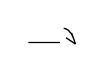
\begin{tikzpicture}[x=1mm,y=1mm]\draw[line width=.45pt] (0,0)--(4,0) (4.5,1.8) to[out=-10,in=110] (6,-.2) (6,-.2)--(5.5,1.2) (6,-.2)--(4.8,.6);\end{tikzpicture}}
\inserted{and if [$\unsure{i|j}\otimes{\mathrm{id}}_{A\otimes A}$ is also one, then the \unsure{condition|condition} \tikz[baseline=(s.base)]{\node[inner sep=1pt](s){\(u_M(M'')\subset\mathrm{Im}\,M''_{\otimes A}\)};\draw[->] ([xshift=-7pt,yshift=10pt]s.north west)--([xshift=-6pt,yshift=-3pt]s.north west)--([xshift=-2pt,yshift=9pt]s.north west);} is necessary and \uline{sufficient} for \deleted{\unsure{stability}} stability ; then $M'$ is \unsure{stable|stable} if and only if $M''$ is.}
% @ 21
\deleted{\unsure{batise|banise} \unsure{these remarks}}. The conditions considered are ok in the following cases :

% @ 22
a) $A$ is flat$/k$ (for~example $k$ a field)

% @ 22–24 right margin
\margin{\deleted{Then the \unsure{c.s.} of \unsure{the} \unsure{question} \unsure{apply} \unsure{show} $u_M(M'')\subset\mathrm{Im}\,M''_{\otimes A}$.} 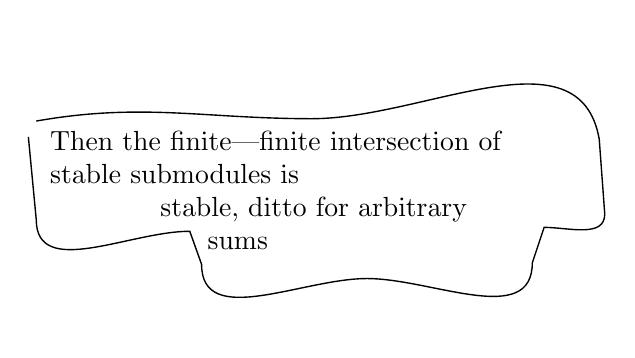
\begin{tikzpicture}[x=1cm,y=1cm]\node[anchor=north west,align=left,text width=7cm,inner sep=2pt](s) at (0,0){Then the \unsure{\deleted{finite}|finite} intersection of\\stable submodules is\\\hspace*{1.4cm}stable, ditto for arbitrary\\\hspace*{2cm}sums};\draw[line width=.5pt] (-.1,.05) to[out=10,in=180] (3.4,.08) to[out=0,in=100] (7.05,-.18)--(7.12,-1.13) to[out=-90,in=0] (6.35,-1.3)--(6.2,-1.75) to[out=-90,in=0] (4.1,-1.95) to[out=180,in=-90] (2,-1.77)--(1.85,-1.35) to[out=180,in=-90] (-.1,-1.2)--(-.2,-.15);\end{tikzpicture}}
% @ 23
b) $M/M''$ is \inserted{$\unsure{A|\wedge}$}-flat

% @ 24
c) $M''$ a direct summand in $M$.

% @ 24 left margin
% slanted
\margin{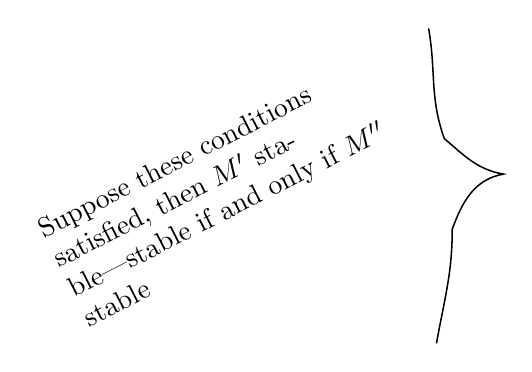
\begin{tikzpicture}[x=1cm,y=1cm]\node[rotate=27,align=left,text width=4.5cm,inner sep=2pt](s) at (0,0){\deleted{Suppose these conditions satisfied, then $M'$ \unsure{stable|stable} if and only if $M''$ stable}};\draw[line width=.55pt] (2.65,2.1) to[out=-80,in=110] (2.85,.7) to[out=-40,in=170] (3.6,.25) to[out=190,in=70] (2.95,-.45) to[out=-90,in=80] (2.75,-1.9);\end{tikzpicture}}
% @ 25
\deleted{or $A$ \unsure{free well}.}

% @ 26–29
In the case $A$ free [more generally a sum of finitely generated projective modules] one sees that $M'$ is \unsure{stable|stable} if and only if $M'$ is \deleted{stable under the action of $\check{A}$.} a sub-$\check{A}$-module. One therefore finds

% @ 30–32
\uline{Proposition} If $A$ is a sum of finitely generated projective modules, then a sub-$k$-module \deleted{of} $A$-comodule is stable if and only if it is \deleted{stable under the action} \unsure{a|is} sub $\unsure{\check{A}|\tilde{A}}$-module.
% archive sheet number: 28
